\label{porting}
Vector Pascal is an open-source project. It aims to create
a productive an efficient program development environment for
SIMD programming. In order to validate the concepts it has
been developed initially for the Intel family of processors
running Linux and Microsoft Windows. However it has been intended
from the outset that the technology should be portable to other
families of CPUs. This chapter addresses some of the issues
involved in porting the compiler to new systems.

\section{Dependencies}

The Vector Pascal compiler tool-set can be divided along two axes
as shown in figure \ref{toolset}. \begin{enumerate}
\item Tools can be divided into (a) those provided as part of the release , versus (b) tools provided
      as part of the operating environment.
     \begin{enumerate}
	\item These are mainly written in Java, the exceptions being a  small run-time
              library in C, a Pascal System unit, and several machine descriptions.
        \item These are all available as standard under Linux, and Windows versions
              are freely downloadable from the web.
     \end{enumerate}
\item Tools can further divided into (a) those required for program preparation
and documentation, (b) code translation tools, and (c) code generator preparation tools.
     \begin{enumerate}
       \item The program preparation tools are the VIPER IDE described in Chapter \ref{vipintro},
       along with the standard \LaTeX document prepartion system, DVI viewers, and the
       TTH tool to prepare web enabled versions of Vector Pascal program descriptions.
       \item The program translation tools are:
            \begin{enumerate}
             \item The {\tt ilcg.pascal} Java package which
             contains the Pascal compiler itself and classes to support Pascal type
             declarations. This carries out the first stage of code translation, from
             Pascal to an ILCG tree\cite{Cockshott00}.
             \item A set of machine generated code generators for CPUs such as the Pentium,
              the K6 etc. These carry out the second phase of code translation - into
              an assembler file.
             \item The {\tt ilcg.tree} Java package which supports the internal representation
                   of ILCG trees (see section \ref{ilcgintro}).
             \item The Java system which is need to run all of the above.
             \item An assembler, which is necessary to carry out the third phase
                   of code translation, from an assembler file to a relocatable
                   object file.
             \item A C compiler and linkage system is needed to compile the C run-time
                   library and to link the relocatable object files into final executables.
			\item If compiling to a GPU, Nvidias nvcc is needed.
             \item In addition if one wants to alter the reserved words of Vector Pascal
                   or make other lexical changes one needs the JLex lexical analyser
                   generator.

            \end{enumerate}
     \end{enumerate}

\end{enumerate}

\begin{figure}%[h]
\epsfig{file=toolset.eps,width=4.6in}
\caption{Vector Pascal toolset}\label{toolset}
\end{figure}


\section{Compiler Structure}

\begin{figure}[h]\center
\epsfig{file=system.eps,width=3.5in}
\caption{The translation of Vector Pascal to assembler.}\label{system}
\end{figure}
The structure of the  Vector Pascal translation
 system is shown in figure \ref{fig:system}.
The main program class of the compiler {\tt ilcg.Pascal.PascalCompiler.java} translates
the source code of the program into an internal structure called an ILCG tree
\cite{Cockshott00}. A machine generated code generator then translates this
into assembler code. An example would be the class ilcg.tree.IA32. An assembler
and linker specified in descendent class of the code generator then translate
the assembler code into an executable file.



 Consider first the path followed from a source file, the phases that it goes through are
\begin{itemize}
\item[i.] The source file (1) is parsed by a java class PascalCompiler.class (2) a   
hand written, recursive descent parser\cite{Watt}, and results
in a Java data structure (3), an ILCG tree, which is basically a semantic
tree for the program. %The classes from which this is built are from package {\tt ilcg.tree}.
\item[ii.] The resulting tree is transformed (4) from sequential to parallel form
and  machine independent optimisations are performed.
Since ILCG trees
 are java objects, they can contain methods to self-optimise. Each class
contains for instance a method {\tt eval} which attempts to evaluate a tree at
compile time. Another method {\tt simplify} applies generic machine
independent transpormations to the code. Thus the {\tt simplify}
method of the class {\tt For} can perform loop unrolling,
removal of redundant loops etc. Other methods allow tree walkers
to apply context specific transformations.
\item[iii.] The resulting ilcg tree (7) is walked over by a class that encapsulates
the semantics of the target machine's instructionset (10); for example Pentium.class.
During code generation the tree is futher transformed, as machine
specific register optimisations are performed. 
The output of this process is an assembler file (11).
\item[iv.] This is then fed through an appropriate assembler and linker, assumed
to be externally provided to generate an executable program.
\end{itemize}

\subsection{Vectorisation}

The parser initially generates serial code for all constructs.
It then interogates the current code generator class to determine
the degree of parallelism possible for the types of operations performed
in a loop, and if these are greater than one, it vectorises the code.

Given the declaration 

{\bf var v1,v2,v3:array[1..9] of integer;}

then the statement

{\bf v1:=v2+v3;}

would first be translated to the ILCG sequence shown in figure \ref{seqf}
\begin{figure}
\begin{verbatim}
{ var  i;
  for  i=1 to 9 step 1 do {
   v1[^i]:= +(^(v2[^i]),^(v3[^i]));
  };
}
\end{verbatim}
\caption{Sequential form of array assignment}\label{seqf}
\end{figure}
In the example above variable names such as {\tt v1} and {\tt i} have been used
for clarity. In reality {\tt i} would be an addressing expression like:

\verb{ (ref int32)mem(+(^((ref int32)ebp),     -1860)){,

which encodes both the type and the address of the variable.
The code generator is queried as to the parallelism available on
the type {\tt int32} and, since it is a Pentium with MMX, returns
2.
The loop is then split into two, a portion that can be executed in
parallel and a residual sequential component, resulting in the 
ILCG shown in figure \ref{parf}.\begin{figure}\begin{verbatim}
{ var i;  
   for i=    1 to     8 step     2 do {
    (ref int32 vector ( 2 ))mem(+(@v1,*(-(^i,1),4))):=
       +(^((ref int32 vector ( 2 ))mem(+(@v2,*(-(^i,1),4)))), 
         ^((ref int32 vector ( 2 ))mem(+(@v3,*(-(^i,1),4)))));
   };
   for i=    9 to     9 step     1 do {
      v1[^i]:= +(^(v2[^i]),^(v3[^i]));
   };
}
\end{verbatim}
\caption{Parallelised loop}\label{parf}
\end{figure}
In the parallel part of the code, the array subscriptions have been replaced
by explictly cast memory addresses. This coerces the locations from their
original types to the type required by the vectorisation.
Applying the {\tt simplify } method of the For class  the
following generic transformations are performed:
\begin{enumerate}
\item The second loop is replaced by a single statement.
\item The parallel loop is unrolled twofold.
\item The For class is replaced by a sequence of statements with
explicit gotos.
\end{enumerate}
The result is shown in figure \ref{simpf}.
When the {\tt eval} method is invoked, 
constant folding causes the loop test condition
to be evaluated  to

\verb{if >(^i,8) then	goto leb4af11b47f{.
\begin{figure}
\begin{verbatim}
{ var i:
  i:= 1;
  leb4af11b47e:
  if >( 2, 0) then	if >(^i,8) then	goto leb4af11b47f
	                else null
                        fi
         else if <(^i, 8) then	goto leb4af11b47f
         else null
         fi
  fi;
 (ref int32 vector ( 2 ))mem(+(@v1,*(-(^i,1),4))):=
       +(^((ref int32 vector ( 2 ))mem(+(@v2,*(-(^i,1),4)))), 
         ^((ref int32 vector ( 2 ))mem(+(@v3,*(-(^i,1),4)))));
  i:=+(^i,2);
 (ref int32 vector ( 2 ))mem(+(@v1,*(-(^i,1),4))):=
       +(^((ref int32 vector ( 2 ))mem(+(@v2,*(-(^i,1),4)))), 
         ^((ref int32 vector ( 2 ))mem(+(@v3,*(-(^i,1),4)))));
  i:=+(^i,2);
  goto leb4af11b47e;
  leb4af11b47f:
  i:=    9;
  v1[^i]:= +(^(v2[^i]),^(v3[^i]));
}
\end{verbatim}
\caption{After applying {\tt simplify} to the tree}
\label{simpf} 
\end{figure}

\begin{figure}
\begin{verbatim}
 mov DWORD ecx,     1
leb4b08729615: 
 cmp DWORD ecx,      8
 jg near  leb4b08729616
 lea edi,[  ecx-(     1)]; substituting in edi with 3 occurences  
 movq MM1, [  ebp+edi* 4+     -1620]
 paddd MM1, [  ebp+edi* 4+     -1640]
 movq  [  ebp+edi* 4+     -1600],MM1
 lea ecx,[  ecx+     2]
 lea edi,[  ecx-(     1)]; substituting in edi with 3 occurences  
 movq MM1, [  ebp+edi* 4+     -1620]
 paddd MM1, [  ebp+edi* 4+     -1640]
 movq  [  ebp+edi* 4+     -1600],MM1
 lea ecx,[  ecx+     2]
 jmp  leb4b08729615
leb4b08729616:
\end{verbatim}
\caption{The result of matching the parallelised loop against the Pentium
instruction set}\label{matchf}
\end{figure}

\subsection{Porting strategy}
To port the compiler to a new machine, say a G5, it is necessary to 

\begin{enumerate}
\item Write a new machine description \texttt{G5.ilc} in ILCG source code.
\item Compile this to a code generator in java with the ilcg compiler generator using
a command of the form

\begin{enumerate}
\item \texttt{java ilcg.ILCG cpus/G5.ilc ilcg/tree/G5.java G5}
\end{enumerate}
\item Write an interface class {\tt ilcg/tree/G5CG} which is a subclass of 
{\tt G5 } and which
invokes the assembler and linker. The linker and assembler used will depend
on the machine but one can assume that at least a {\tt gcc} assembler and
linker will be available. The class {\tt G5CG} must take responsibility to
handle the translation of procedure calls from the abstract form provided
in ILCG to the concrete form required by the G5 processor.
\item
The class {\tt G5CG} should also export the method {\tt getparallelism}
which specifies to the vectoriser the degree of parallelism available
for given data types. An example for a P4 is given in figure \ref{getparallelism}.
Note that although a P4 is potentially capable of performing 16 way 
parallelism on 8 bit operands the measured speed  when doing this 
on is less than that measured for 8 way parallelism. This is due
to the restriction placed on un-aligned loads of 16 byte quantities
in the P4 architecture. For image processing operations aligned accesses
are the exception. Thus when specifying
the degree of parallelism for a processor one should not simply give
the maximal degree supported by the architecture. The maximal level
of parallelism is not necessarily the fastest.
\end{enumerate}
\begin{figure}
\begin{verbatim}
public int getParallelism(String elementType) 
{   if(elementType.equals(Node.int32)) return 2;
    if(elementType.equals(Node.int16)) return 4;
    if(elementType.equals(Node.int8)) return 8;   
    if(elementType.equals(Node.uint32)) return 2;
    if(elementType.equals(Node.uint16)) return 4;
    if(elementType.equals(Node.uint8)) return 8;  
    if(elementType.equals(Node.ieee32))return 4; 
    if(elementType.equals(Node.ieee64))return 1;  
    return 1; 
} 
\end{verbatim}
\caption{The method getParallelism for a P4 processor.
   }
\label{getparallelism}
\end{figure}
Sample machine descriptions for the Pentium and 486  are given in chapter \ref{machines}
to help
those wishing to port the compiler.  
These are given in the  ILCG machine description language, an outline of which follows.



\section{ILCG }\label{ilcgintro}
The purpose of ILCG (Intermediate Language for Code Generation) is to 
mediate between CPU instruction sets and high level language programs.
It poth provides a representation to which compilers can translate
a variety of source level programming languages and also a notation for
defining the semantics of CPU instructions.


Its purpose is to act as an input to two types of programs:
\begin{enumerate}\item ILCG structures produced by a HLL compiler are input to 
an automatically constructed code generator,
working on the syntax matching principles described in \cite{graham80}. This then
generates equivalent sequences of assembler statements.
\item Machine descriptions written as ILCG source files are input to
code-generator-generators which produce java programs which perform function (1)
above.
\end{enumerate}
So far one HLL compiler producing ILCG structures as output
exists: the Vector Pascal compiler.
There also exists one code-generator-generator which produces code generators
that use a top-down pattern matching technique analogous to Prolog unification.
%It is assumed that all store allocation appart from register spillage has already been accomplished.

ILCG is   intended to be flexible enough to describe a wide variety of machine
architectures. In particular it can specify both SISD and SIMD instructions and
either stack-based or register-based machines.
 However, it does assume certain
things about the machine:  that certain basic types are supported and that
the machine is addressed at the byte level.

In ILCG all type conversions, dereferences etc have to be made
absolutely explicit.
%Since the notation is intended primarily to be machine generated we are
%concerned with human readability, and thus use a prefix notation.

In what follows we will designate terminals of the language in bold thus {\bf octet}
and nonterminal in sloping font thus {\sl word8}.
\section{Supported types}
\subsection{Data formats}
The data in a memory can be distinguished initially in terms of the number of bits
in the individually addressable chunks. The addressable chunks are assumed to be the
powers of two from 3 to 7, so we thus have as allowed formats:{\sl word8, word16, word32, word64,
word128}.
These are treated as non terminals in the grammar of ILCG.

When data is being explicitly operated on without regard to its type, we have terminals which
stand for these formats: {\bf octet, halfword, word, doubleword, quadword}.
\subsection{Typed formats}
Each of these underlying formats can contain information of different types, either
signed or unsigned integers, floats etc.
ILCG allows the following integer types as terminals :{\bf
int8, uint8, int16, uint16, int32, uint32, int64, uint64 }to stand for signed and
unsigned integers of the appropriate lengths.

The integers are logically grouped into {\sl signed} and {\sl unsigned}.
As non-terminal types they are represented as 
{\sl byte, short, integer, long} and
{\sl ubyte, ushort, uinteger, ulong}.

Floating point numbers are either assumed to be 32 bit or 64 bit with 32 bit numbers
given the nonterminal symbols {\sl float,double}. If we wish to specify a particular
representation of floats of doubles we can use the terminals {\bf ieee32, ieee64}.



\subsection{Ref types}
ILCG uses a simplified version of the Algol-68 reference typing model.
A value can be a reference to another type. Thus an integer when used as
an address of a 64 bit floating point number would be a {\bf ref ieee64 }.
Ref types include registers. An integer register would be a {\bf ref int32}
when holding an integer, a {\bf ref ref int32} when holding the address
of an integer etc.
\section{Supported operations}
\subsection{Type casts}



The syntax for the type casts is C style so we have
for example {\tt (ieee64) int32} to represent a conversion
of an 32 bit integer to a 64 bit real. These type casts
act as constraints on the pattern matcher during code 
generation. They do not perform any data transformation.
They are inserted into machine descritions to constrain the
types of the arguments that will be matched for an instruction.
They are also used by compilers to decorate ILCG trees 
in order both to enforce, and to allow limited breaking of, the type rules. 

\subsection{Arithmetic}
The allowed dyadic arithmetic operations are addition, saturated addition, multiplication,
saturated multiplication,
subtraction, saturated subtraction,
division and remainder with operator symboles {\bf +, +:, *, *:, -, -:, div , mod}.. 
 

The concrete syntax is prefix with bracketing. Thus 
the infix operation $ 3+5 \div 7$ would be
represented as {\bf +(3 div (5 7))}.
\subsection{Memory}
Memory is explicitly represented. All accesses to memory are
represented by array operations on a predefined array {\bf mem}.
Thus location 100 in memory is represented as {\bf mem(100)}.
The type of such an expression is {\sl address}.
It can be cast to a reference type of a given format.
Thus we could have
{\bf

(ref int32)mem(100)
}

\subsection{ Assignment }
We have a set of storage  operators corresponding to the
word lengths supported. These  have the form of 
infix operators. The size of the store being performed
depends on the size of the right hand side.
A valid storage statement might be 
{\bf

(ref octet)mem( 299) :=(int8) 99

}
The first argument is always a reference and the second 
argument a value of the appropriate format.

If the left hand side is a format the right hand side
must be a value of the appropriate size.
If the left hand side is an explicit type rather than
a format, the right hand side must have the same type.
\subsection{ Dereferencing}
Dereferencing is done explicitly when a value other than a literal is required.
There is a dereference operator, which converts a reference 
into the value that it references.
 A valid load expression might be:
{\bf

(octet)$\uparrow$  ( (ref octet)mem(99))

}
The argument to the load operator must be a reference.

\section{Machine description}
Ilcg can be used to describe the semantics of machine instructions.
A machine description typically consists of a set of register declarations
followed by a set of instruction formats and a set of operations.
This approach works well only with machines that have an orthogonal
instruction set, ie, those that allow addressing modes and operators
to be combined in an independent manner.
\subsection{Registers }
When entering machine descriptions in ilcg registers can be declared
along with their type hence
{\bf

register word EBX assembles['ebx'] ;

reserved register word ESP assembles['esp'];
 

}
would declare {\bf EBX} to be of type {\bf ref word}.

\subsubsection{Aliasing}
A register can be declared to be a sub-field of another register,
hence we could write 
{\bf

 alias register octet AL = EAX(0:7) assembles['al']; 

 alias register octet BL = EBX(0:7) assembles['bl'];


}
to indicate that {\bf BL} occupies the bottom 8 bits of register {\bf EBX}.
In this notation bit zero is taken to be the least significant bit of a value.
There are assumed to be two pregiven registers {\bf FP, GP} that
are used by compilers to point to  areas of memory.
These can be aliased to a particular real register.{\bf

register word EBP assembles['ebp'] ;

alias register word FP = EBP(0:31) assembles ['ebp'];

}

Additional registers may be reserved, indicating that the code generator
must not use them to hold temporary values:

{\bf

reserved register word ESP assembles['esp'];
}
 
\subsection{Register sets}
A set of registers that are used in the same way by the instructionset
can be defined.
{\bf

pattern reg means [$ EBP| EBX|ESI|EDI|ECX |EAX|EDX|ESP$]  ;

pattern breg means[$ AL|AH|BL|BH|CL|CH|DL|DH$];
}

All registers in an register set should be of the same length.


\subsection{Register Arrays}
Some machine designs have regular arrays of registers.
Rather than have these exhaustively enumerated it is convenient to
have a means of providing an array of registers.
This can be declared as:


{\bf

register  vector(8)doubleword MM assembles['MM'i] ;

}
 
 
This declares the symbol MMX to stand for the entire MMX register
set. It implicitly defines how the register names are to be
printed in the assembly language by defining an indexing variable
i that is used in the assembly language definition.

We also need a syntax for explicitly identifying individual
registers in the set. This is done by using
the dyadic subscript operator:
{\bf

subscript(MM,2)

}
which would be of type {\bf ref doubleword}.
\subsection{Register Stacks}
Whilst some machines have registers organised as an array,
another class of machines, those oriented around postfix instructionsets,
have register stacks.

The ilcg syntax allows register stacks to be declared:



{\bf

register stack (8)ieee64 FP assembles[ ' '] ;


}

Two access operations are supported on stacks:
\paragraph{PUSH} is a void dyadic operator taking a stack of type ref $t$ as first argument
and a value of  type $t$ as the second argument. Thus we might have:
{ \bf

PUSH(FP,$\uparrow$mem(20))
}

\paragraph{POP} is a monadic operator returning $t$ on stacks of type $t$. So we might have
{\bf

mem(20):=POP(FP)
} 
In addition there are two predicates on stacks that can be used in pattern pre-conditions.
\paragraph{FULL} is a monadic boolean operator on stacks.
\paragraph{EMPTY} is a monadic boolean operator on stacks.
\subsection{Instruction formats}

An instruction format is an abstraction over a class of concrete instructions.
It abstracts over particular operations
 and types thereof
whilst specifying how arguments can be combined.
{\bf

instruction pattern 

RR( operator op, anyreg r1, anyreg r2, int t)

        means[r1:=(t) op( $\uparrow$((ref t) r1),$\uparrow$((ref t) r2))]    

	assembles[op ' ' r1 ',' r2];


}
In the above example, we specify a register to register instruction format
that uses the first register as a source and a destination whilst the second
register is only a destination. The 
 result is returned in register r1.


We might however wish to have a more powerful abstraction, which was capable of
taking more abstract apecifications for its arguments. For example, many machines
allow arguments to instructions to be addressing modes that can be either
registers or memory references. For us to be able to specify this in an instruction
format we need to be able to provide grammer non-terminals as arguments
to the instruction formats.

For example we might want to be able to say

{\bf

instruction  pattern 

RRM(operator op, reg r1, maddrmode rm, int t)

        means [r1:=(t) op( $\uparrow$((ref t)r1),$\uparrow$((ref t) rm))]

        assembles[op ' ' r1 ',' rm ] ;}

This implies that addrmode and reg must be non terminals.
Since the non terminals required by different machines will vary, there
must be a means of declaring such non-terminals in ilcg.

An example would be:
{
\bf 

 


 pattern regindirf(reg r) 

	means[$\uparrow$(r) ]
	assembles[ r ];

pattern baseplusoffsetf(reg r, signed s) 

	means[+(  $\uparrow$(r) ,const s)]
	assembles[  r '+' s ];

pattern addrform means[baseplusoffsetf$|$ regindirf];

 

pattern maddrmode(addrform f) 

means[mem(f) ] assembles[ '[' f ']' ];

}
This gives us a way of including non terminals as parameters to patterns.




\section{Grammar of ILCG}
The following grammar is given in Sable \cite{sable} compatible form.
The Sable parser generator is used to generate a parser for ILCG from
this grammar. The ILCG parser then translates a CPU specification into
a tree structure which is then walked by an ILCG-tree-walk-generator
to produce an ILCG-tree-walk Java class specific to that CPU.

If the ILCG grammar is extended, for example to allow new arithmetic
operators, then the ILCG-tree-walk-generator must itself be modified
to generate translation rules for the new operators.

\small
\input ilcggram
\normalsize
\chapter{Sample Machine Descriptions}\label{machines}
 \small
\section{Basic 386 architecture}
\input{../../cpus/i386base.m4}
%\section{The x87 Floating Point Processor}
%\input{../../cpus/ifpu.m4}
\section{The MMX instruction-set}
\input{../../cpus/mmx.m4}
\section{The 486 CPU}
\input{../../cpus/ia32.m4}

\input{../../cpus/pentium.m4}
 \normalsize
\subsection{Concrete representation}


